%%
% Copyright (c) 2017 - 2023, Pascal Wagler;
% Copyright (c) 2014 - 2023, John MacFarlane
%
% All rights reserved.
%
% Redistribution and use in source and binary forms, with or without
% modification, are permitted provided that the following conditions
% are met:
%
% - Redistributions of source code must retain the above copyright
% notice, this list of conditions and the following disclaimer.
%
% - Redistributions in binary form must reproduce the above copyright
% notice, this list of conditions and the following disclaimer in the
% documentation and/or other materials provided with the distribution.
%
% - Neither the name of John MacFarlane nor the names of other
% contributors may be used to endorse or promote products derived
% from this software without specific prior written permission.
%
% THIS SOFTWARE IS PROVIDED BY THE COPYRIGHT HOLDERS AND CONTRIBUTORS
% "AS IS" AND ANY EXPRESS OR IMPLIED WARRANTIES, INCLUDING, BUT NOT
% LIMITED TO, THE IMPLIED WARRANTIES OF MERCHANTABILITY AND FITNESS
% FOR A PARTICULAR PURPOSE ARE DISCLAIMED. IN NO EVENT SHALL THE
% COPYRIGHT OWNER OR CONTRIBUTORS BE LIABLE FOR ANY DIRECT, INDIRECT,
% INCIDENTAL, SPECIAL, EXEMPLARY, OR CONSEQUENTIAL DAMAGES (INCLUDING,
% BUT NOT LIMITED TO, PROCUREMENT OF SUBSTITUTE GOODS OR SERVICES;
% LOSS OF USE, DATA, OR PROFITS; OR BUSINESS INTERRUPTION) HOWEVER
% CAUSED AND ON ANY THEORY OF LIABILITY, WHETHER IN CONTRACT, STRICT
% LIABILITY, OR TORT (INCLUDING NEGLIGENCE OR OTHERWISE) ARISING IN
% ANY WAY OUT OF THE USE OF THIS SOFTWARE, EVEN IF ADVISED OF THE
% POSSIBILITY OF SUCH DAMAGE.
%%

%%
% This is the Eisvogel pandoc LaTeX template.
%
% For usage information and examples visit the official GitHub page:
% https://github.com/Wandmalfarbe/pandoc-latex-template
%%

% Options for packages loaded elsewhere
\PassOptionsToPackage{unicode}{hyperref}
\PassOptionsToPackage{hyphens}{url}
\PassOptionsToPackage{dvipsnames,svgnames,x11names,table}{xcolor}
%
\documentclass[
  paper=a4,
  ,captions=tableheading
]{scrartcl}
\usepackage{amsmath,amssymb}
% Use setspace anyway because we change the default line spacing.
% The spacing is changed early to affect the titlepage and the TOC.
\usepackage{setspace}
\setstretch{1.2}
\usepackage{iftex}
\ifPDFTeX
  \usepackage[T1]{fontenc}
  \usepackage[utf8]{inputenc}
  \usepackage{textcomp} % provide euro and other symbols
\else % if luatex or xetex
  \usepackage{unicode-math} % this also loads fontspec
  \defaultfontfeatures{Scale=MatchLowercase}
  \defaultfontfeatures[\rmfamily]{Ligatures=TeX,Scale=1}
\fi
\usepackage{lmodern}
\ifPDFTeX\else
  % xetex/luatex font selection
\fi
% Use upquote if available, for straight quotes in verbatim environments
\IfFileExists{upquote.sty}{\usepackage{upquote}}{}
\IfFileExists{microtype.sty}{% use microtype if available
  \usepackage[]{microtype}
  \UseMicrotypeSet[protrusion]{basicmath} % disable protrusion for tt fonts
}{}
\makeatletter
\@ifundefined{KOMAClassName}{% if non-KOMA class
  \IfFileExists{parskip.sty}{%
    \usepackage{parskip}
  }{% else
    \setlength{\parindent}{0pt}
    \setlength{\parskip}{6pt plus 2pt minus 1pt}}
}{% if KOMA class
  \KOMAoptions{parskip=half}}
\makeatother
\usepackage{xcolor}
\definecolor{default-linkcolor}{HTML}{A50000}
\definecolor{default-filecolor}{HTML}{A50000}
\definecolor{default-citecolor}{HTML}{4077C0}
\definecolor{default-urlcolor}{HTML}{4077C0}
\usepackage[margin=2.5cm,includehead=true,includefoot=true,centering,]{geometry}
% add backlinks to footnote references, cf. https://tex.stackexchange.com/questions/302266/make-footnote-clickable-both-ways
\usepackage{footnotebackref}
\usepackage{graphicx}
\makeatletter
\def\maxwidth{\ifdim\Gin@nat@width>\linewidth\linewidth\else\Gin@nat@width\fi}
\def\maxheight{\ifdim\Gin@nat@height>\textheight\textheight\else\Gin@nat@height\fi}
\makeatother
% Scale images if necessary, so that they will not overflow the page
% margins by default, and it is still possible to overwrite the defaults
% using explicit options in \includegraphics[width, height, ...]{}
\setkeys{Gin}{width=\maxwidth,height=\maxheight,keepaspectratio}
% Set default figure placement to htbp
\makeatletter
% Make use of float-package and set default placement for figures to H.
% The option H means 'PUT IT HERE' (as  opposed to the standard h option which means 'You may put it here if you like').
\usepackage{float}
\floatplacement{figure}{H}
\makeatother
\setlength{\emergencystretch}{3em} % prevent overfull lines
\providecommand{\tightlist}{%
  \setlength{\itemsep}{0pt}\setlength{\parskip}{0pt}}
\setcounter{secnumdepth}{-\maxdimen} % remove section numbering
\ifLuaTeX
\usepackage[bidi=basic]{babel}
\else
\usepackage[bidi=default]{babel}
\fi
\babelprovide[main,import]{french}
% get rid of language-specific shorthands (see #6817):
\let\LanguageShortHands\languageshorthands
\def\languageshorthands#1{}
\ifLuaTeX
  \usepackage{selnolig}  % disable illegal ligatures
\fi
\IfFileExists{bookmark.sty}{\usepackage{bookmark}}{\usepackage{hyperref}}
\IfFileExists{xurl.sty}{\usepackage{xurl}}{} % add URL line breaks if available
\urlstyle{same}
\hypersetup{
  pdftitle={Enquêtes de conjoncture auprès des entreprises},
  pdfauthor={@statjunior},
  pdflang={fr-FR},
  hidelinks,
  breaklinks=true,
  pdfcreator={LaTeX via pandoc with the Eisvogel template}}
\title{Enquêtes de conjoncture auprès des entreprises}
\usepackage{etoolbox}
\makeatletter
\providecommand{\subtitle}[1]{% add subtitle to \maketitle
  \apptocmd{\@title}{\par {\large #1 \par}}{}{}
}
\makeatother
\subtitle{Résultats au mois de juillet 2023}
\author{@statjunior}
\date{20 juillet 2023}



%%
%% added
%%


%
% for the background color of the title page
%
\usepackage{pagecolor}
\usepackage{afterpage}
\usepackage[margin=2.5cm,includehead=true,includefoot=true,centering]{geometry}

%
% break urls
%
\PassOptionsToPackage{hyphens}{url}

%
% When using babel or polyglossia with biblatex, loading csquotes is recommended
% to ensure that quoted texts are typeset according to the rules of your main language.
%
\usepackage{csquotes}

%
% captions
%
\definecolor{caption-color}{HTML}{777777}
\usepackage[font={stretch=1.2}, textfont={color=caption-color}, position=top, skip=4mm, labelfont=bf, singlelinecheck=false, justification=raggedright]{caption}
\setcapindent{0em}

%
% blockquote
%
\definecolor{blockquote-border}{RGB}{221,221,221}
\definecolor{blockquote-text}{RGB}{119,119,119}
\usepackage{mdframed}
\newmdenv[rightline=false,bottomline=false,topline=false,linewidth=3pt,linecolor=blockquote-border,skipabove=\parskip]{customblockquote}
\renewenvironment{quote}{\begin{customblockquote}\list{}{\rightmargin=0em\leftmargin=0em}%
\item\relax\color{blockquote-text}\ignorespaces}{\unskip\unskip\endlist\end{customblockquote}}

%
% Source Sans Pro as the default font family
% Source Code Pro for monospace text
%
% 'default' option sets the default
% font family to Source Sans Pro, not \sfdefault.
%
\ifnum 0\ifxetex 1\fi\ifluatex 1\fi=0 % if pdftex
    \usepackage[default]{sourcesanspro}
  \usepackage{sourcecodepro}
  \else % if not pdftex
    \usepackage[default]{sourcesanspro}
  \usepackage{sourcecodepro}

  % XeLaTeX specific adjustments for straight quotes: https://tex.stackexchange.com/a/354887
  % This issue is already fixed (see https://github.com/silkeh/latex-sourcecodepro/pull/5) but the
  % fix is still unreleased.
  % TODO: Remove this workaround when the new version of sourcecodepro is released on CTAN.
  \ifxetex
    \makeatletter
    \defaultfontfeatures[\ttfamily]
      { Numbers   = \sourcecodepro@figurestyle,
        Scale     = \SourceCodePro@scale,
        Extension = .otf }
    \setmonofont
      [ UprightFont    = *-\sourcecodepro@regstyle,
        ItalicFont     = *-\sourcecodepro@regstyle It,
        BoldFont       = *-\sourcecodepro@boldstyle,
        BoldItalicFont = *-\sourcecodepro@boldstyle It ]
      {SourceCodePro}
    \makeatother
  \fi
  \fi

%
% heading color
%
\definecolor{heading-color}{RGB}{40,40,40}
\addtokomafont{section}{\color{heading-color}}
% When using the classes report, scrreprt, book,
% scrbook or memoir, uncomment the following line.
%\addtokomafont{chapter}{\color{heading-color}}

%
% variables for title, author and date
%
\usepackage{titling}
\title{Enquêtes de conjoncture auprès des entreprises}
\author{@statjunior}
\date{20 juillet 2023}

%
% tables
%

%
% remove paragraph indention
%
\setlength{\parindent}{0pt}
\setlength{\parskip}{6pt plus 2pt minus 1pt}
\setlength{\emergencystretch}{3em}  % prevent overfull lines

%
%
% Listings
%
%


%
% header and footer
%

%%
%% end added
%%

\begin{document}

%%
%% begin titlepage
%%
\begin{titlepage}
\newgeometry{left=6cm}
\definecolor{titlepage-color}{HTML}{884373}
\newpagecolor{titlepage-color}\afterpage{\restorepagecolor}
\newcommand{\colorRule}[3][black]{\textcolor[HTML]{#1}{\rule{#2}{#3}}}
\begin{flushleft}
\noindent
\\[-1em]
\color[HTML]{FFFFFF}
\makebox[0pt][l]{\colorRule[435488]{1.3\textwidth}{4pt}}
\par
\noindent

{
  \setstretch{1.4}
  \vfill
  \noindent {\huge \textbf{\textsf{Enquêtes de conjoncture auprès des
entreprises}}}
    \vskip 1em
  {\Large \textsf{Résultats au mois de juillet 2023}}
    \vskip 2em
  \noindent {\Large \textsf{@statjunior}}
  \vfill
}


\textsf{20 juillet 2023}
\end{flushleft}
\end{titlepage}
\restoregeometry
\pagenumbering{arabic} 

%%
%% end titlepage
%%

% \maketitle


\hypertarget{pruxe9sentation}{%
\section{Présentation}\label{pruxe9sentation}}

Ce rapport \emph{RMarkdown} présente les résultats des enquêtes de
conjoncture auprès des entreprises réalisées par l'Insee. Le dernier
point connu est juillet 2023.

On présente tout d'abord l'indicateur synthétique du climat des affaires
ainsi que celui de l'emploi pour tous les secteurs de l'économie. Cet
indicateur est de moyenne 100 sur longue période (et d'écart-type 10).

On s'intéresse ensuite au climat des affaires par secteur d'activité
(bâtiment, industrie manufacturière, commerce de détail, services). On
présente également les évolutions de prix et d'emploi prévues par les
chefs d'entreprise de chaque secteur, à un horizon de court-terme.

Enfin, on analyse plus spécifiquement les difficultés de production
présentes dans l'industrie manufacturière, en distinguant les
contraintes d'offre des contraintes de demande.

Ce rapport a été compilé automatiquement avec le logiciel \texttt{R}, le
20 juillet 2023 à 11 heures et 35 minutes. Les potentielles erreurs
présentes dans ce document relèvent uniquement de la responsabilité de
Statjunior.

Le code source permettant de générer ce document est disponible sur Git
\href{https://github.com/statjunior/Statjunior/tree/main/Enqu\%C3\%AAtes\%20de\%20conjoncture/}{en
cliquant ici}.

\hypertarget{climat-conjoncturel-global}{%
\section{Climat conjoncturel global}\label{climat-conjoncturel-global}}

\hypertarget{climat-des-affaires-et-de-lemploi}{%
\subsection{Climat des affaires et de
l'emploi}\label{climat-des-affaires-et-de-lemploi}}

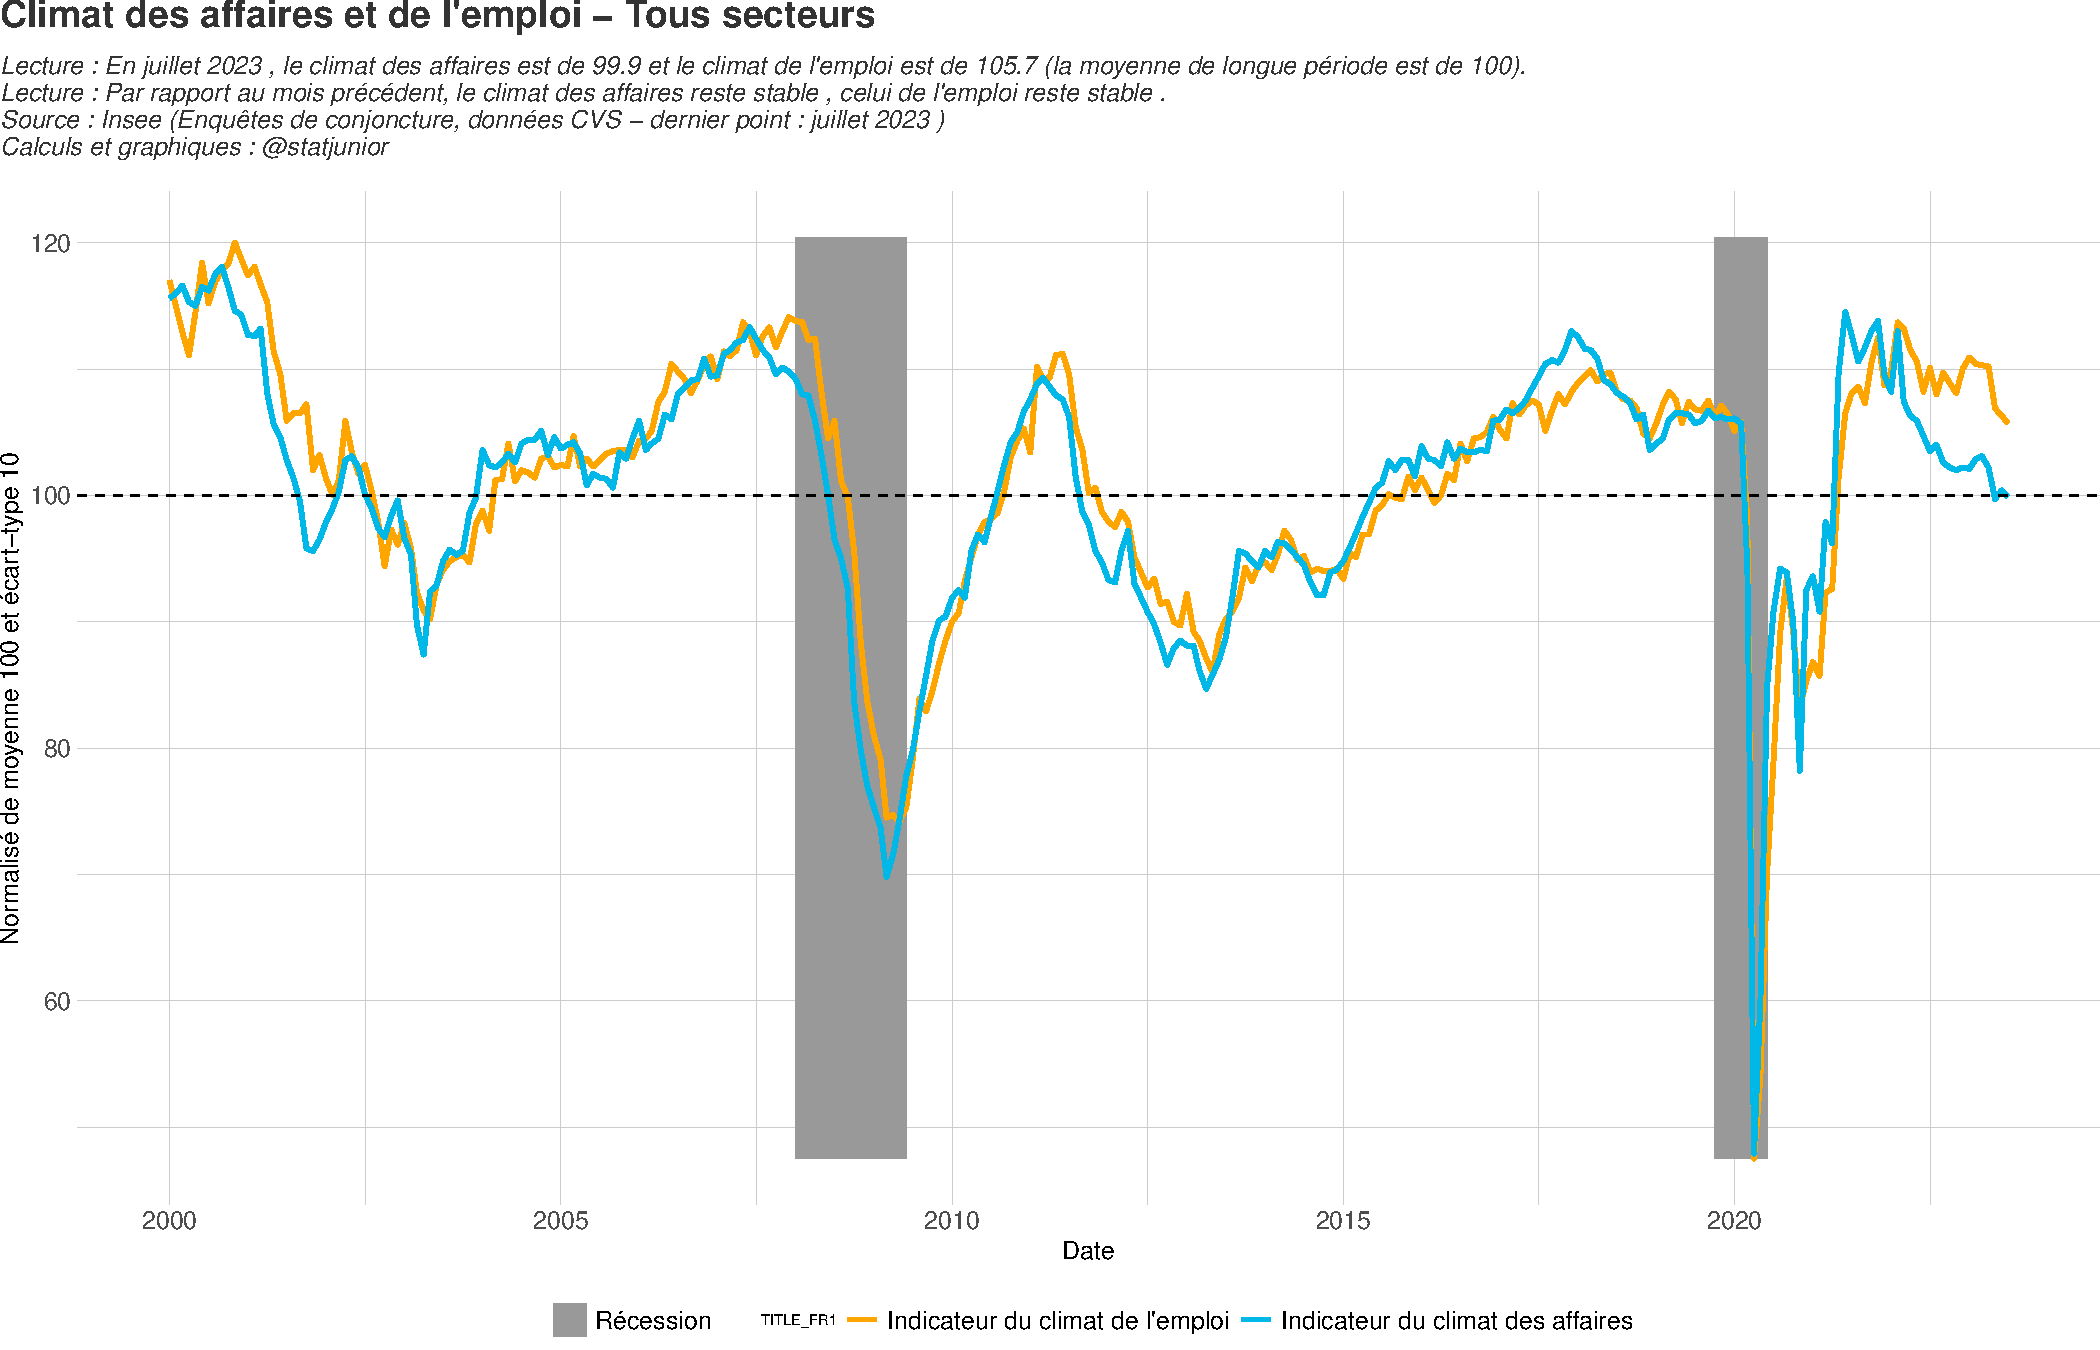
\includegraphics{rapport_pdf_enquete_conj_files/figure-latex/unnamed-chunk-2-1.pdf}

\hypertarget{indicateur-de-retournement-conjoncturel}{%
\subsection{Indicateur de retournement
conjoncturel}\label{indicateur-de-retournement-conjoncturel}}

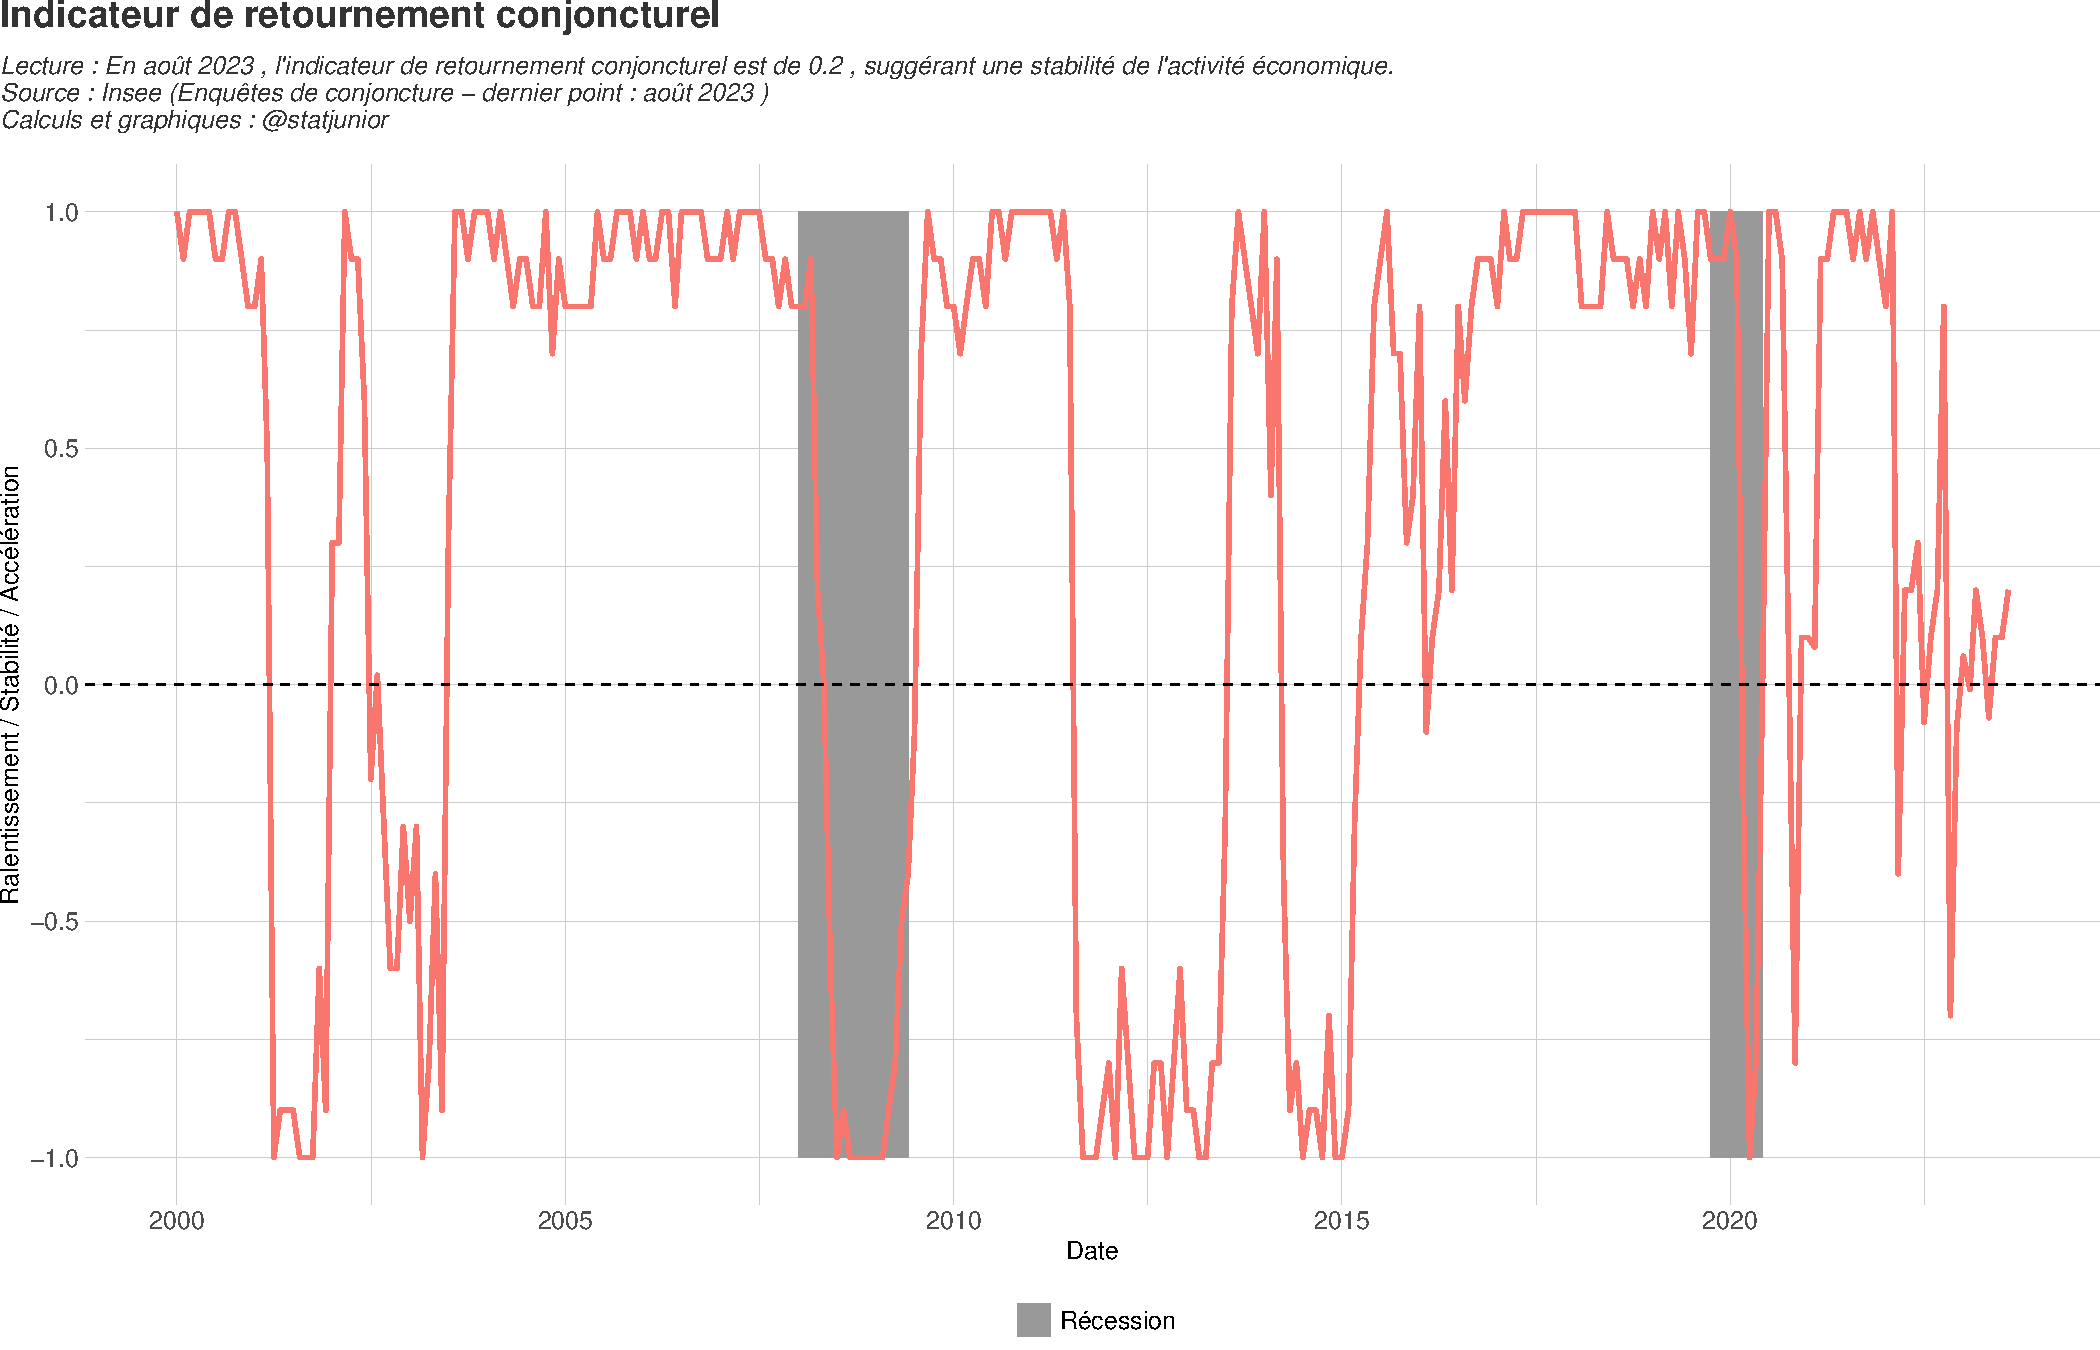
\includegraphics{rapport_pdf_enquete_conj_files/figure-latex/unnamed-chunk-3-1.pdf}

\hypertarget{climat-conjoncturel-sectoriel}{%
\section{Climat conjoncturel
sectoriel}\label{climat-conjoncturel-sectoriel}}

\hypertarget{climat-des-affaires-par-secteur}{%
\subsection{Climat des affaires par
secteur}\label{climat-des-affaires-par-secteur}}

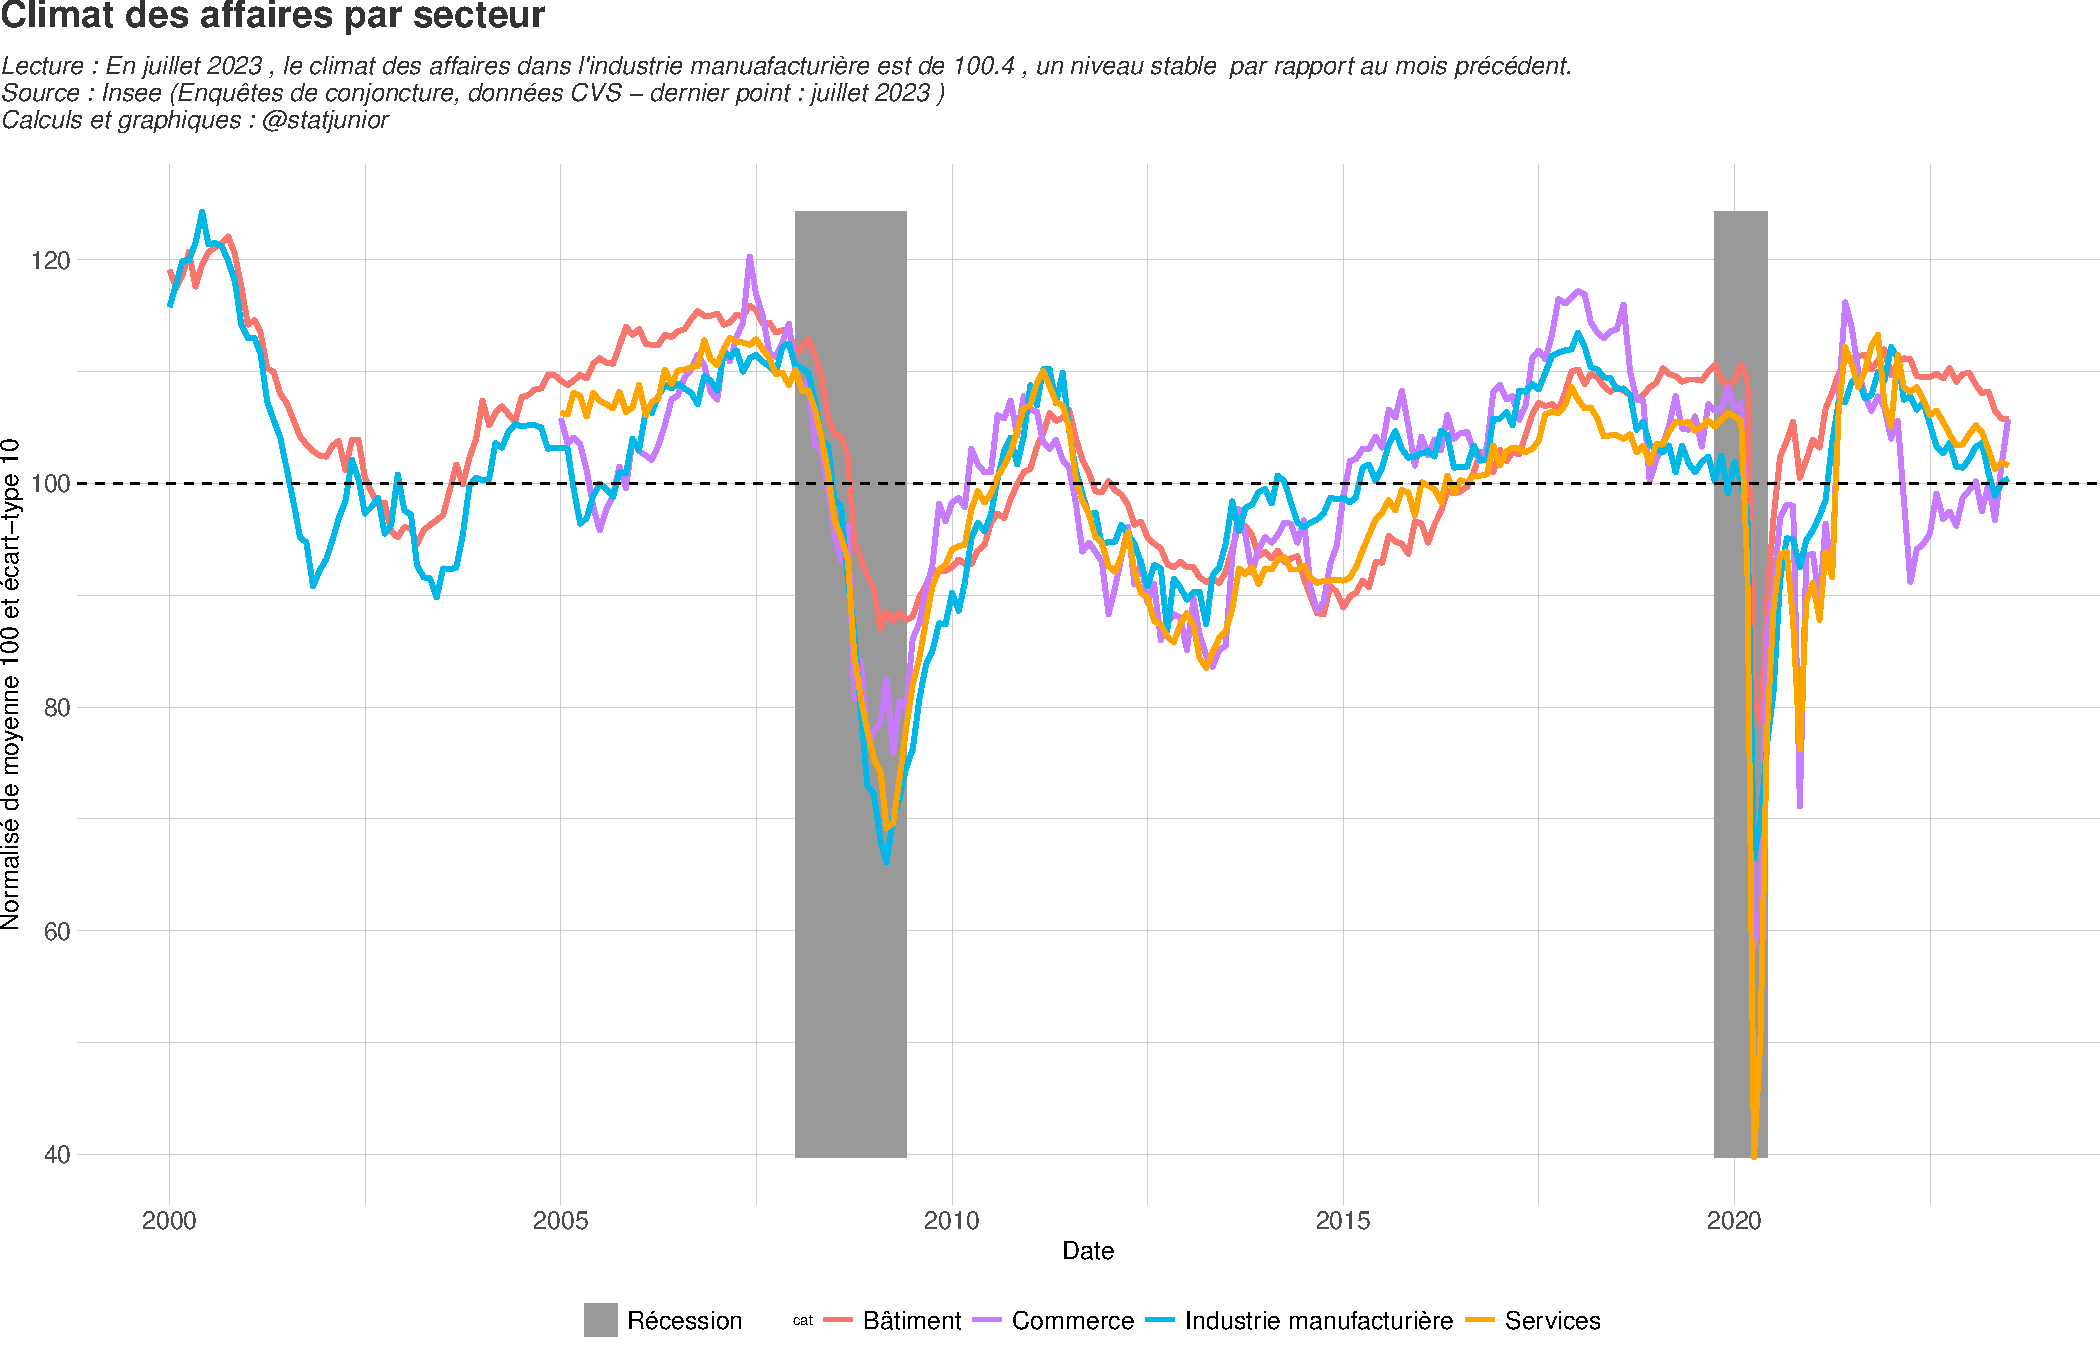
\includegraphics{rapport_pdf_enquete_conj_files/figure-latex/unnamed-chunk-5-1.pdf}

\hypertarget{evolution-des-prix-pruxe9vue-par-secteur}{%
\subsection{Evolution des prix prévue par
secteur}\label{evolution-des-prix-pruxe9vue-par-secteur}}

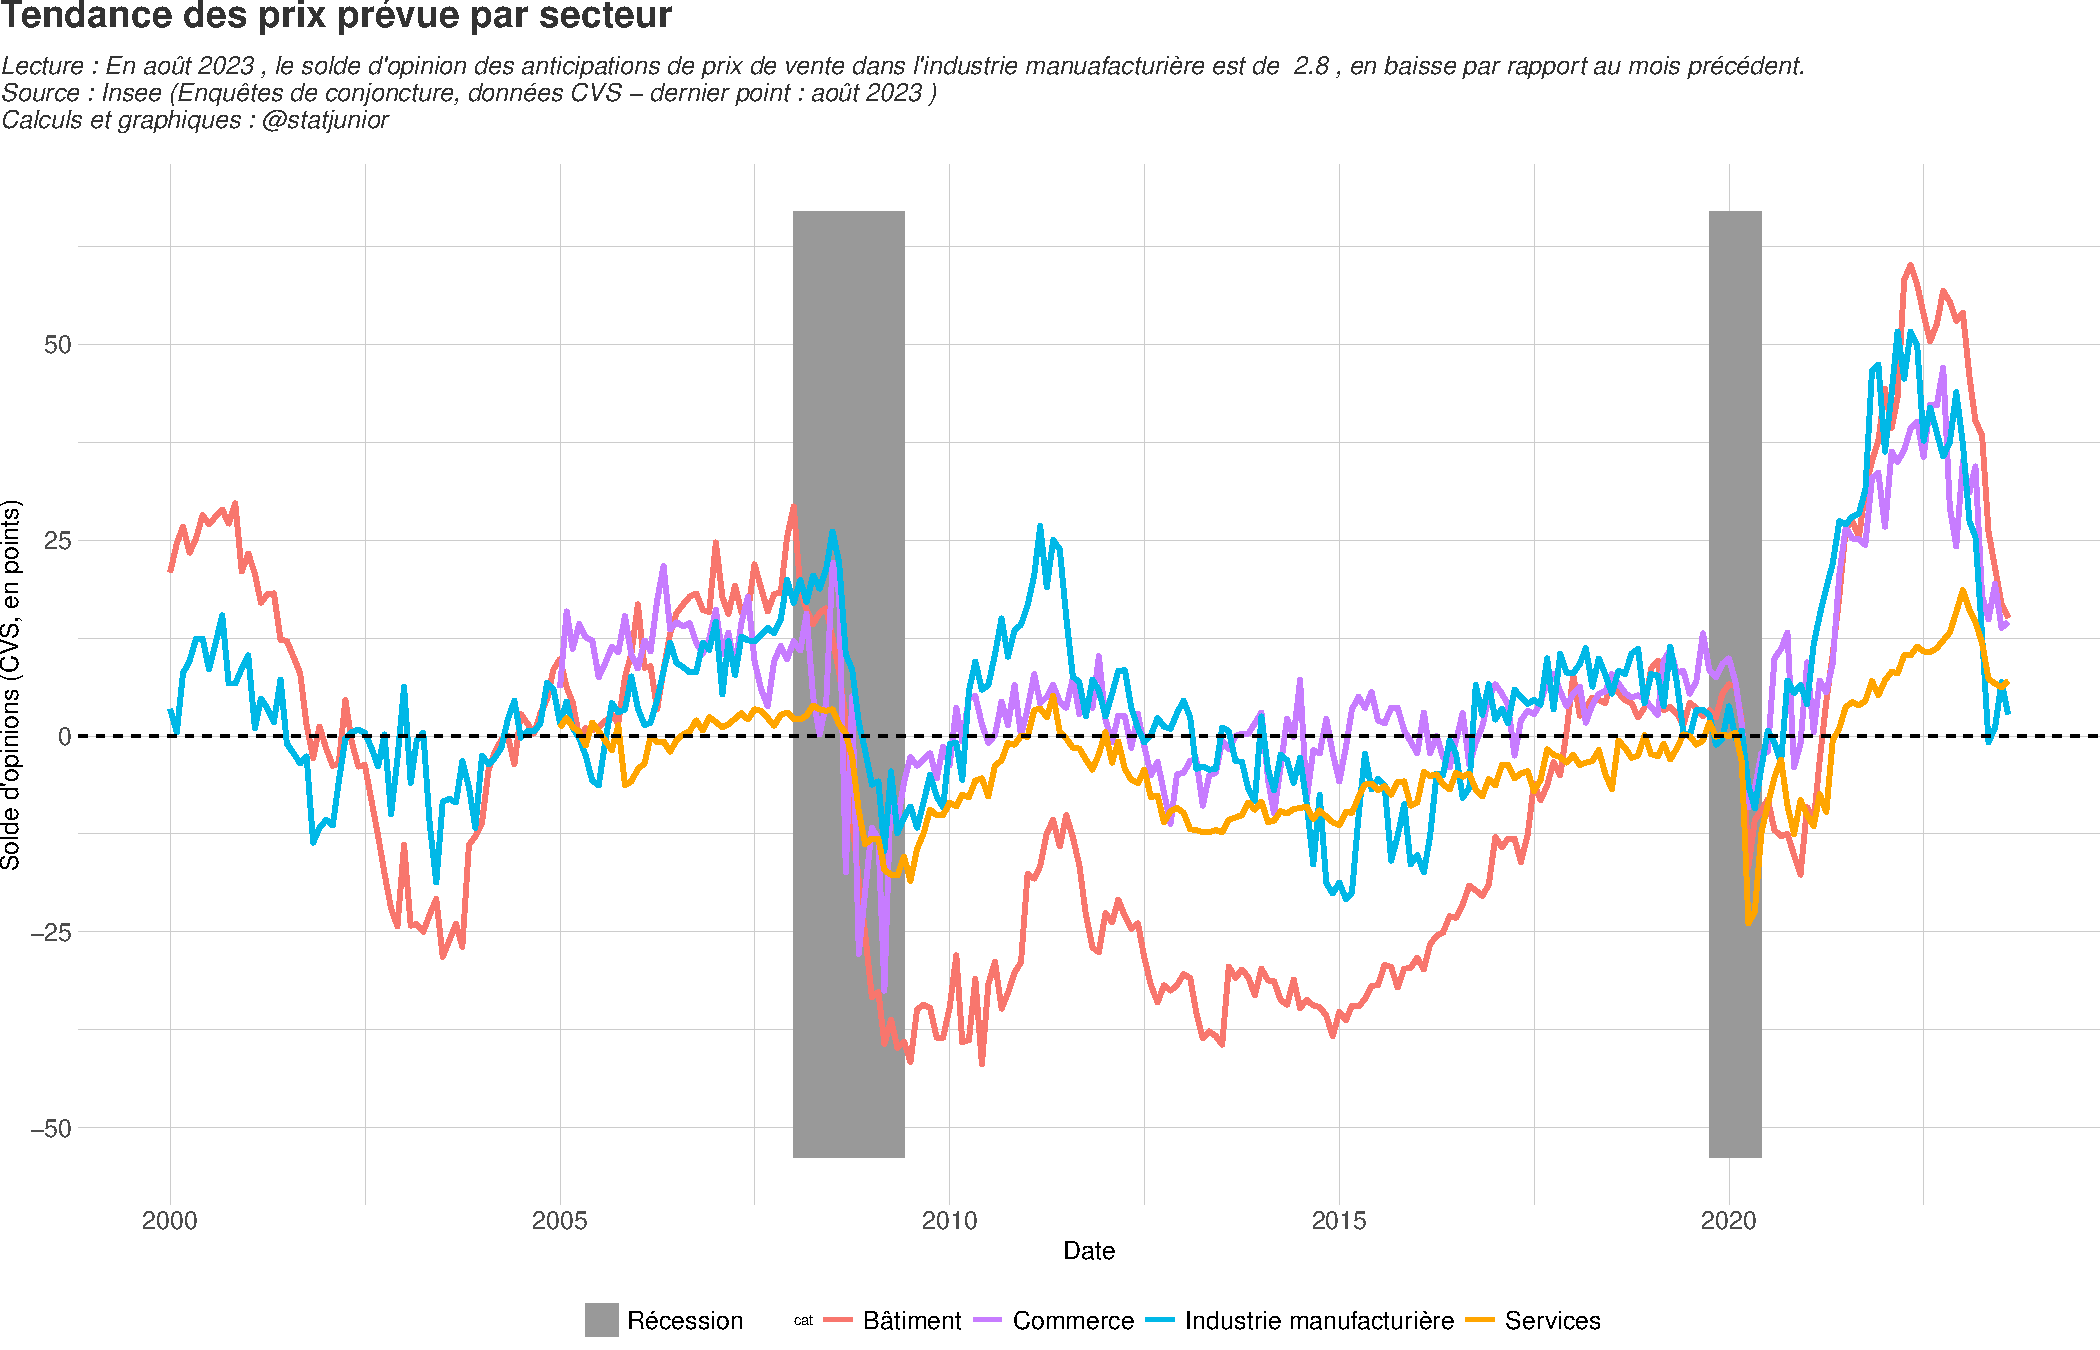
\includegraphics{rapport_pdf_enquete_conj_files/figure-latex/unnamed-chunk-6-1.pdf}

\hypertarget{evolution-de-lemploi-pruxe9vue-par-secteur}{%
\subsection{Evolution de l'emploi prévue par
secteur}\label{evolution-de-lemploi-pruxe9vue-par-secteur}}

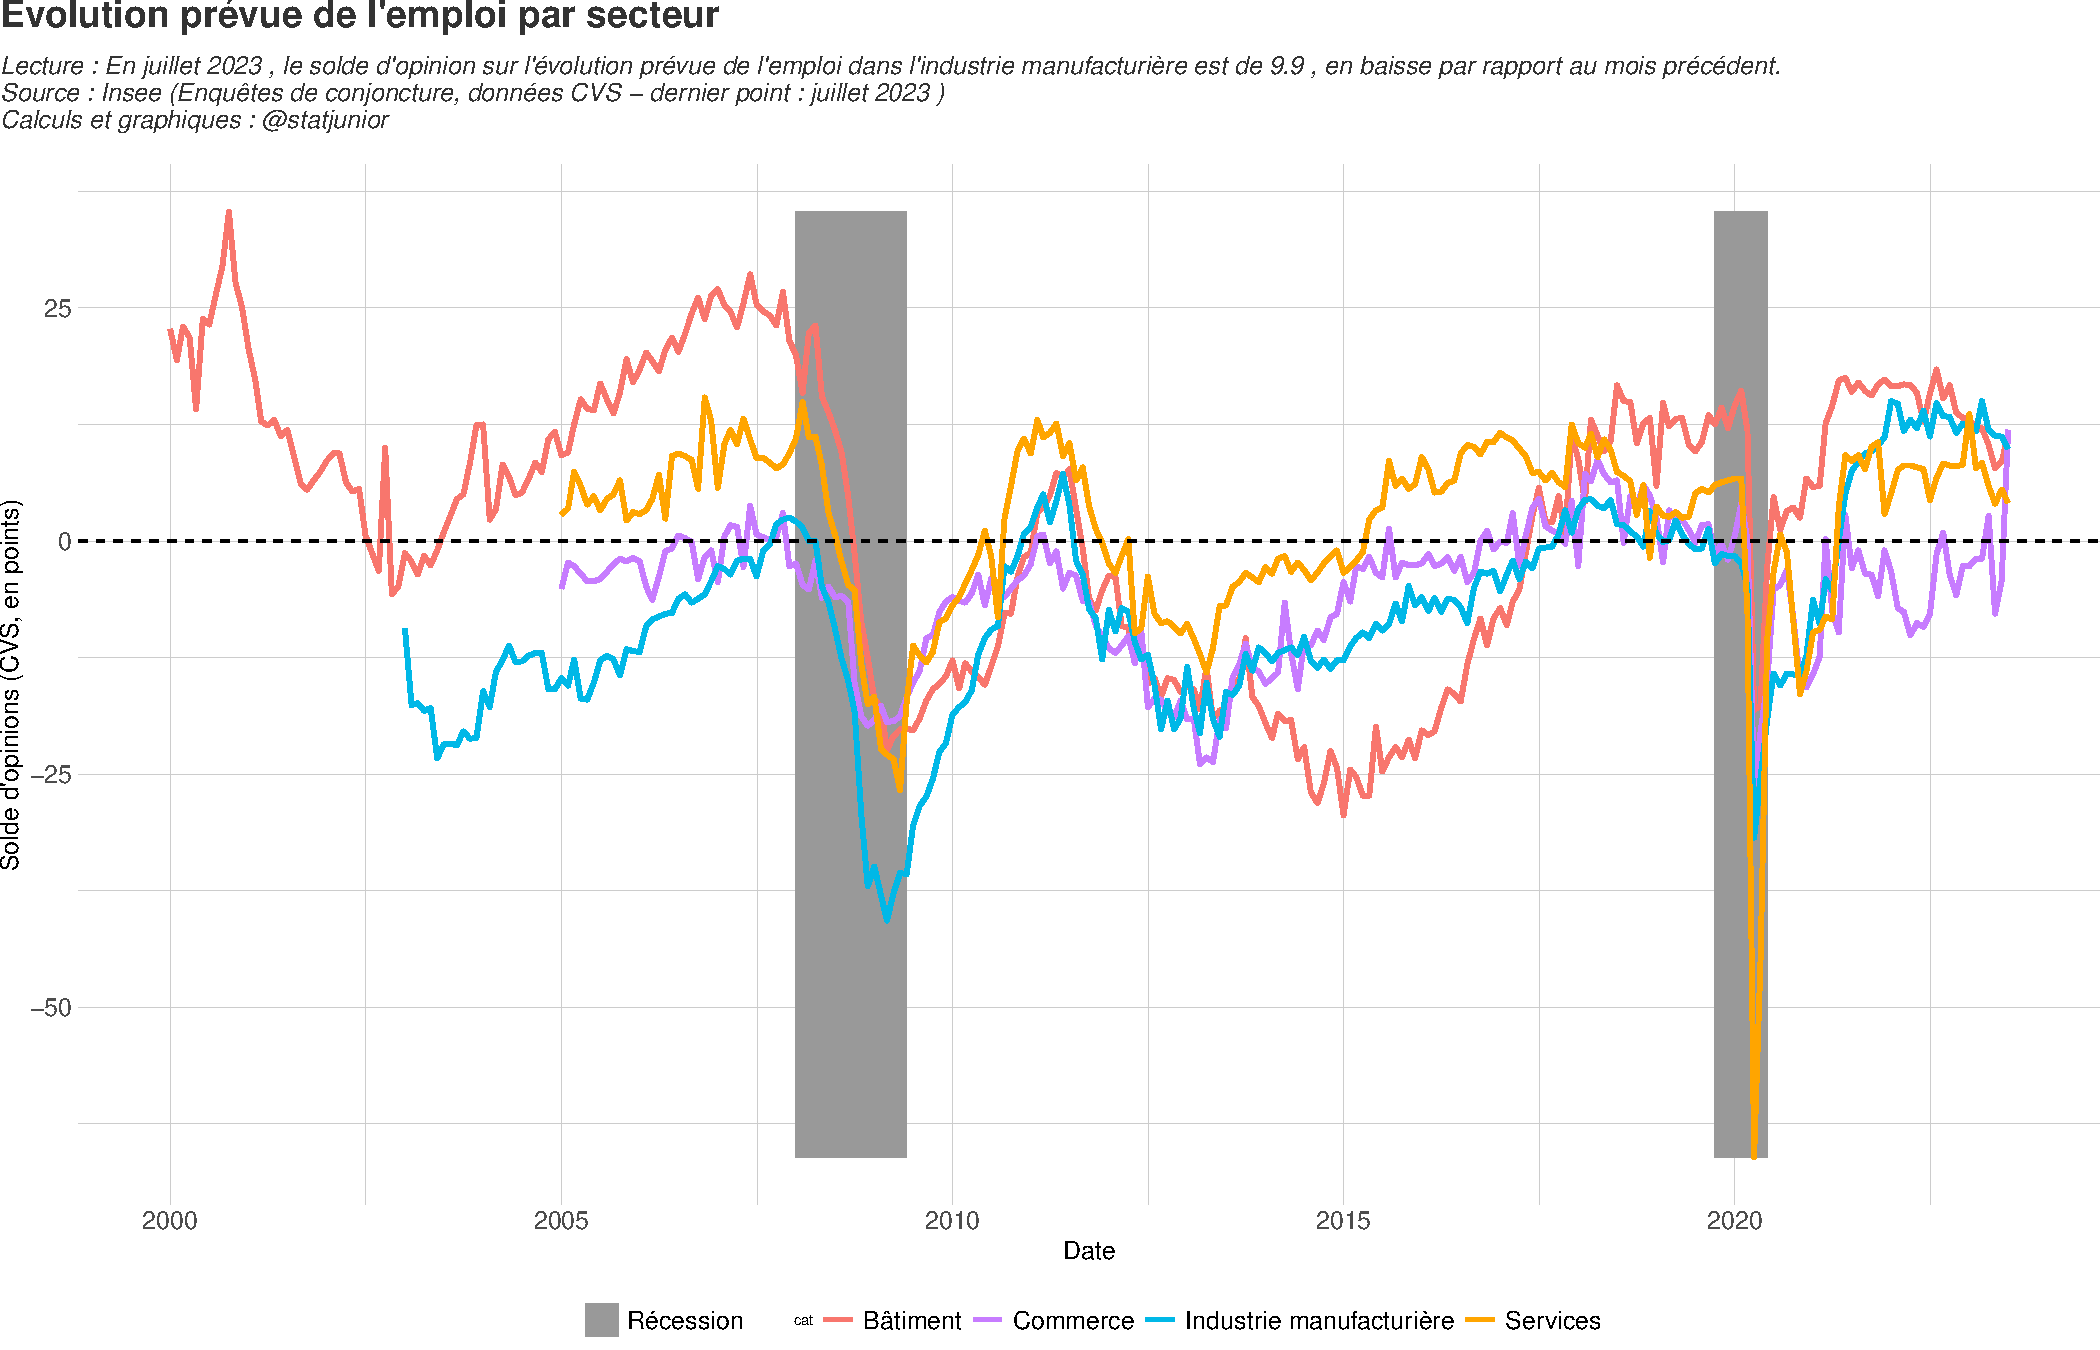
\includegraphics{rapport_pdf_enquete_conj_files/figure-latex/unnamed-chunk-7-1.pdf}

\hypertarget{contraintes-de-production-dans-lindustrie}{%
\section{Contraintes de production dans
l'industrie}\label{contraintes-de-production-dans-lindustrie}}

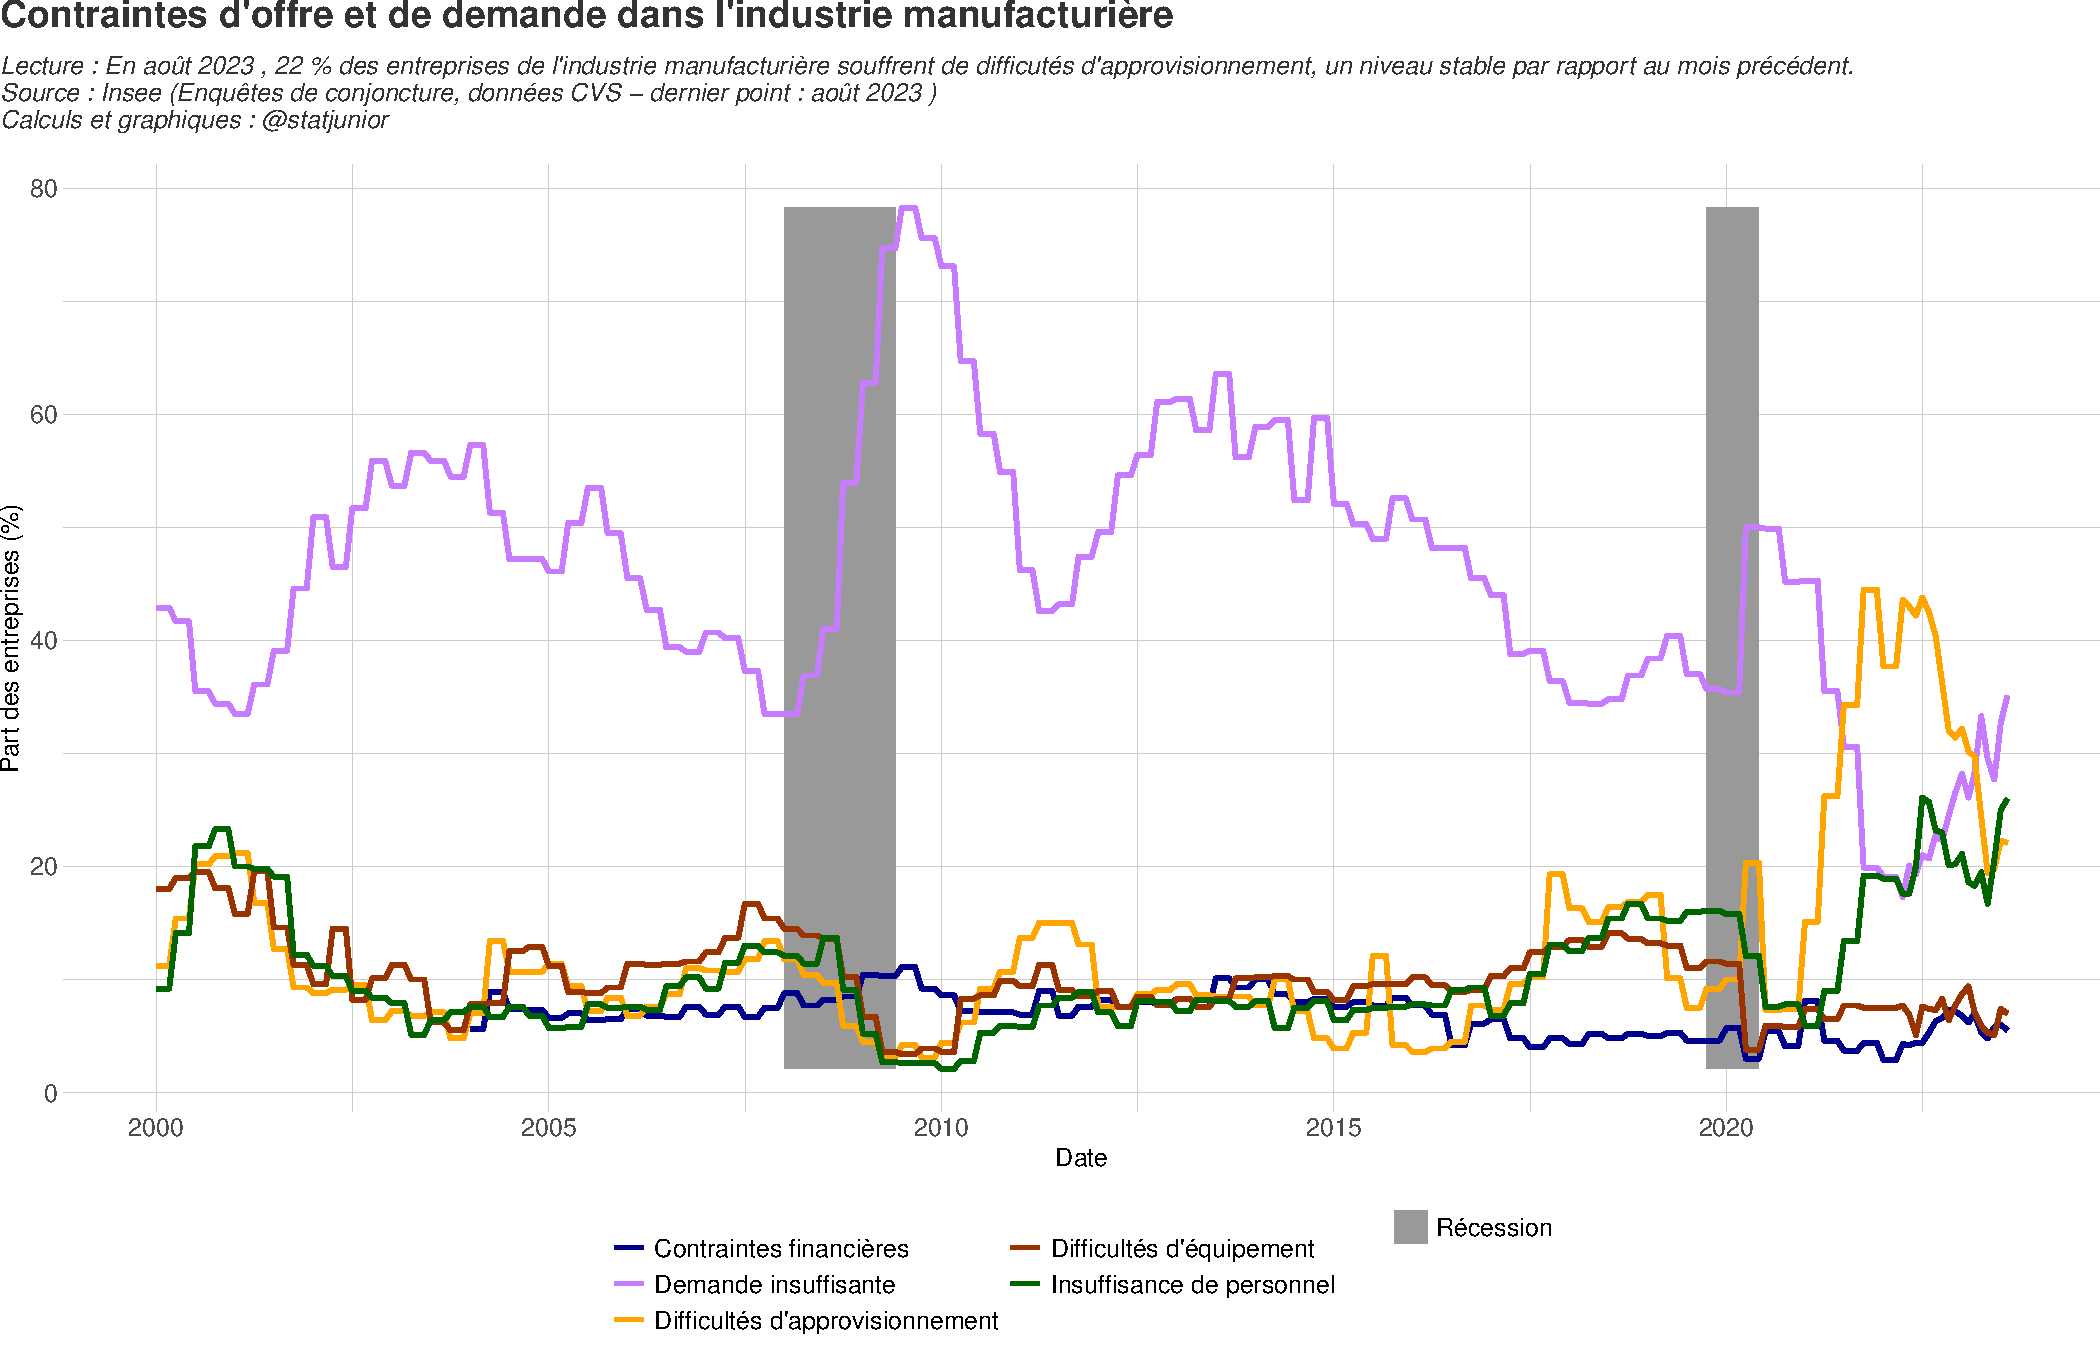
\includegraphics{rapport_pdf_enquete_conj_files/figure-latex/unnamed-chunk-8-1.pdf}

\end{document}
